\section{实验验证与分析}

本节首先阐述评估指标,随后在T-LESS\cite{tless}和IC-BIN\cite{icbin}数据集上,将本方法与现有基于模型的方法进行对比测试。这两个数据集具有以下特性:1) 包含丰富的对称目标类别;2) 存在因纹理失配导致的合成-真实域差异。这些特性使其成为评估对称物体处理方法的理想基准。此外,通过超参数消融实验与可视化效果展示,直观揭示SymCode算法对各关键模块的影响机制。

\subsection{数据集}

\par 在T-LESS数据集\cite{tless}上对该方法进行了全面评估,并与现有的基于模型的方法进行了对比分析。T-LESS数据集是一个用于评估对称物体姿态估计性能的基准数据集,其特点在于包含30个工业相关的无纹理对称物体。这些物体具有以下显著特性:首先,它们缺乏显著的纹理特征或辨别颜色,这使得传统的基于纹理匹配的方法难以有效工作;其次,这些物体展示了高度的对称性和形态相似性,其中部分物体还具有复合结构,这为姿态估计带来了额外的挑战。由于这些物体的对称性,T-LESS数据集特别适合评估方法在对称物体上的表现。
\par T-LESS数据集使用了两种不同的RGB-D传感器进行数据采集:一种是基于结构光技术的Primesense CARMINE 1.09传感器,另一种是基于飞行时间技术的Microsoft Kinect v2传感器。数据集中的测试图像涵盖了从简单场景到复杂场景的多种情况。简单场景包含少量孤立的物体,而复杂场景则包含多个物体实例,并伴有显著的背景杂乱和物体间的遮挡现象。整个数据集包含了来自20个不同场景的测试图像,每个场景都呈现出不同程度的复杂性,这为评估方法的鲁棒性提供了丰富的实验条件。
\par 考虑到为物体位姿标注真实数据的耗时性,采用了BOP挑战赛\cite{hodan2018bop}提供的公开可用的合成物理渲染(PBR)图像。这些高质量的合成图像使我们能够有效验证仅在合成数据上训练的网络性能。通过这种方式,不仅能够评估该方法在真实场景下的表现,还能够验证其在合成数据上的泛化能力。这一实验设计使得我们能够全面评估该方法在不同数据域下的适应性和鲁棒性。

\subsection{评估指标}

可见表面差异(VSD)评估深度绝对差值低于阈值$\tau=20mm$的可见像素比例,以 $e_{VSD}<0.3$\cite{pitteri2019object}为条件评估正确6D物体位姿的召回率。同时严格遵循BOP挑战赛\cite{hodan2024bop}制定的评估标准,采用三项核心指标:可见表面差异(VSD)、最大对称感知表面距离(MSSD)和最大对称感知投影距离(MSPD)。关于评价指标的详细内容参照\autoref{subsec:评价指标}。

\subsection{与现有方法的对比}

\textbf{T-LESS数据集VSD测试结果 } 如\autoref{tab:tless_vsd}所示,本研究在T-LESS数据集上通过 $e_{VSD}<0.3$ 召回率指标与现有方法进行了对比分析。基于FCOS\cite{fcos}检测器生成的2D检测结果,SymNet展现出显著优势,相较于Pitteri等人\cite{pitteri2019object}在RGB模态下报告的结果,实现了25.0\%的显著提升。需要说明的是,由于BOP评估体系具有更全面的评价维度,近期研究多采用该指标进行方法对比 $e_{VSD}<0.3$ 对比数据较为有限。本实验中,Pitteri等人的研究被选为基准对比对象,因其提供了当前最新的RGB模态评估结果。鉴于原Retina检测器代码已不可用,我们同时纳入CosyPose\cite{labbe2020cosypose}的实验数据,该工作同时报告了BOP指标和 $e_{VSD}<0.3$ 召回率,以增强与早期研究的可比性。值得注意的是,在模型训练策略的对比中,仅使用合成数据训练的模型与结合真实图像训练的模型之间未呈现显著性能差异(平均召回率差值<6\%)。这一现象表明该方法在跨域泛化能力方面具有显著优势,能够有效弥合合成数据与真实场景之间的域间差异。为深入分析模型性能,根据物体对称特性将T-LESSS数据集划分为3个类别,并分别给出各类别的平均评估分数。实验结果表明,SymNet在不同对称类型的物体上均保持稳定的检测性能,最高类别平均召回率达到78.02\%。

\begin{sidewaystable}[t]
        \centering
        \caption{
                T-LESS: Object recall for $err_{vsd} < 0.3$ on all Primesense test scenes. The results for the $30$ objects are grouped based on their symmetry type.
        }
        \begin{tabular}{r| c c c c c c c c}
        \toprule
        Method& \multicolumn{2}{c}{AAE \cite{sundermeyer2018implicit}} & Pix2Pose \cite{park2019pix2pose}& EdgeEnhance \cite{wen2020edge}& Pitteri\cite{pitteri2019object} & CosyPose\cite{labbe2020cosypose}& Ours(pbr) & Ours(pbr+real)\\
        \cmidrule(lr){2-3}\cmidrule(lr){4-4}\cmidrule(lr){5-5}\cmidrule(lr){6-6}\cmidrule(lr){7-7}\cmidrule(lr){8-9}
        Detector&\ \ \ \ SSD\ \ \ \ \  &\ Retina\ &\ \ Retina\ \ &\ \ Retina\ \ & Faster-RCNN & Retina & FCOS(pbr) & FCOS(pbr+real)\\
        Symmetry type& RGB & RGB & RGB &RGB& RGB &RGB-D& RGB &RGB \\
        \midrule
        Asymmetry (3)&25.98&16.95&24.73&28.76&36.533&-&66.36&\textbf{69.47}\\
        Continuous (11)&11.90&17.98&36.27&39.05&46.65&-&61.52&\textbf{63.72}\\
        Discrete (16)&14.45&18.86&25.79&32.77&38.47&-&69.51&\textbf{78.02}\\
        \midrule
        Mean&14.67 &18.35 &29.5&34.67&41.27 &62.6&66.27&\textbf{71.92} \\
        \bottomrule
        \end{tabular}
\label{tab:tless_vsd}
\end{sidewaystable}

% \begin{table*}[t]
%         \centering
%         \caption{
%                 T-LESS: Object recall for $err_{vsd} < 0.3$ on all Primesense test scene. The symbol $^*$ denotes continuous symmetry, while $^{**}$ denotes discrete symmetry type. 
%         }
%         \begin{tabular}{r| c c c c c c c c}
%         \toprule
%         Method& \multicolumn{2}{c}{AAE \cite{sundermeyer2018implicit}} & Pix2Pose \cite{park2019pix2pose}& EdgeEnhance \cite{wen2020edge}& Pitteri\cite{pitteri2019object} & CosyPose\cite{labbe2020cosypose}& Ours(pbr) & Ours(pbr+real)\\
%         \cmidrule(lr){2-3}\cmidrule(lr){4-4}\cmidrule(lr){5-5}\cmidrule(lr){6-6}\cmidrule(lr){7-7}\cmidrule(lr){8-9}
%         Detector&\ \ \ \ \ \ SSD\ \ \ \ \ \  &\ \ Retina\ \  &\ \ Retina\ \ &\ \ Retina\ \ & Faster-RCNN & Retina & FCOS(pbr) & FCOS(pbr+real)\\
%         Input type& RGB & RGB & RGB &RGB& RGB &RGB-D& RGB &RGB \\
%         \midrule
%         $^*$1&5.65 &8.87&38.4& 37.01&26.35 &-&\textbf{37.99} &25.26 \\
%         $^*$2&5.46 &13.22&35.3&29.78 &\textbf{56.14} &-&25.38 &36.43 \\
%         $^*$3&7.05 &12.47&40.9&44.42 &\textbf{83.33} &-&44.59 &39.86 \\
%         $^*$4&4.61 &6.56&26.3&26.71 &32.98 &-&\textbf{42.02} &32.86 \\
%         $^{**}$5&36.45 &34.80 &55.2&56.22&44.54 &-&\textbf{86.26} &85.57 \\
%         $^{**}$6&23.15 &20.24 &31.5&47.49&\textbf{98.33} &-&61.90 &90.77 \\
%         $^{**}$7&15.97 &16.21 &1.1&26.88&87.74 &-&73.49 &\textbf{95.25} \\
%         $^{**}$8&10.86 &19.74 &13.1&22.98&17.09 &-&78.31 &\textbf{98.28} \\
%         $^{**}$9&19.59 &36.21 &33.9&33.84&52.54 &-&88.53 &\textbf{89.88} \\
%         $^{**}$10&10.47 &11.55 &45.8&35.79&5.43 &-&74.21 &\textbf{87.70} \\
%         $^{**}$11&4.35 &6.31 &30.7&23.27&27.97 &-&49.21 &\textbf{53.27} \\
%         $^{**}$12&7.80 &8.15 &30.4&26.25&43.08 &-&71.43 &\textbf{81.15} \\
%         $^*$13&3.30 &4.91 &31.0&27.70&48.54 &-&63.49 &\textbf{69.71} \\
%         $^*$14&2.85 &4.61 &19.5&16.76&42.19 &-&69.31 &\textbf{76.98} \\
%         $^*$15&7.90 &26.71&56.1&35.81 &47.10 &-&66.73 &\textbf{85.98} \\
%         $^*$16&13.06 &21.73 &66.5&59.31&42.18 &-&57.89 &\textbf{64.29} \\
%         $^*$17&41.70 &64.84 &37.9&55.20&56.83 &-&90.67 &\textbf{93.38} \\
%         18&47.17 &14.30 &45.3&60.11&19.31 &-&90.01 &\textbf{91.01} \\
%         $^{**}$19&15.95 &22.46 &21.7&7.49&27.53 &-&59.67 &\textbf{70.44} \\
%         $^{**}$20&2.17 &5.27 &1.9&9.83&32.16 &-&40.28 &\textbf{53.10} \\
%         21&19.77 &17.93 &19.4&13.77&41.19 &-&54.56 &\textbf{62.45} \\
%         22&11.01 &18.63 &9.5&12.4&49.10 &-&54.51 &\textbf{54.96} \\
%         $^{**}$23&7.98 &18.63 &30.7&24.19&26.08 &-&67.62 &\textbf{73.21} \\
%         $^*$24&4.74 &4.23 &18.3&37.37&41.34 &-&\textbf{83.73} &81.89 \\
%         $^{**}$25&21.91 &18.76 &9.5&33.98&44.37 &-&57.34 &\textbf{61.01} \\
%         $^{**}$26&10.04 &12.62 &13.9&42.54&23.80 &-&63.99 &\textbf{64.19} \\
%         $^{**}$27&7.42 &21.13 &24.4&28.14&33.78 &-&86.41 &\textbf{90.28} \\
%         $^{**}$28&21.78 &23.07 &43.0&56.06&35.10 &-&66.17 &\textbf{66.52} \\
%         $^{**}$29&15.33 &26.65 &25.8&49.3&15.92 &-&87.40 &\textbf{87.70} \\
%         $^*$30&34.63 &29.58 &28.8&59.43&36.17 &-&\textbf{94.91} &94.25 \\
%         \midrule
%         Mean&14.67 &18.35 &29.5&34.67&41.27 &62.6&66.27 &\textbf{71.92} \\
%         \bottomrule
%         \end{tabular}
% \label{tab:tless_vsd}
% \end{table*}


\textbf{T-LESS数据集BOP测试结果 } 在T-LESS数据集上的BOP基准测试结果如\autoref{tab:tless_bop}所示。采用BOP挑战赛2023\cite{hodan2024bop}提供的默认检测结果,与完全基于合成数据训练的其他方法进行对比。由于该方法无需依赖耗时的姿态优化步骤,能够直接从每个检测结果中获取姿态,因此运行时间显著优于现有方法。实验表明,该模型在保持与ZebraposeSAT-EffnetB4相当精度的同时,使用更轻量的骨干网络(运行时间仅为后者的三分之一)。需要注意的是,此处的运行时间为单物体实例处理耗时,若采用多物体并行推理策略,整体运行时间可进一步优化。

\begin{sidewaystable}[t]
        \centering
        \caption{
                BOP results on dataset T-LESS. The time is the runtime per image averaged over the dataset.
        }
        \begin{tabular}{l c c c c c c c c}
        \toprule
        6D object pose estimation method &Input type&Training type&$AR$&$AR_{VSD}$&$AR_{MSSD}$&$AR_{MSPD}$&Time(s)\\       %表格第一行,&的位置对齐
        \midrule
        CDPNv2~\cite{li2019cdpn}&RGB&pbr&0.407&0.303&0.338&0.579&1.849 \\
        CosyPose~\cite{labbe2020cosypose}&RGB&pbr&0.640&0.571&0.589&0.761&0.493\\
        EPOS~\cite{hodan2020epos}&RGB&pbr&0.467&0.380&0.403&0.619&1.992 \\
        ZebraPose~\cite{su2022zebrapose}&RGB&pbr&0.677&0.597&0.636&0.466&0.25 \\
        ZebraPoseSAT-EffnetB4~\cite{su2022zebrapose}&RGB&pbr&0.723&0.659&\textbf{0.695}&0.817&0.25 \\
        SurfEmb~\cite{haugaard2022surfemb}&RGB&pbr&0.735&\textbf{0.661}&0.686&0.857&9.043 \\
        SymNet(Ours)&RGB&pbr&\textbf{0.736}&0.631&0.693&\textbf{0.883}&\textbf{0.093} \\
        \midrule
        DPODv2~\cite{shugurov2021dpodv2}&RGB-D&pbr&0.699&0.646&0.716&0.736&0.320 \\
        \midrule
        ZebraPose~\cite{su2022zebrapose}&RGB&real+pbr&0.775&0.696&0.740&0.889&0.25 \\
        SymNet(Ours)&RGB&real+pbr&0.767&0.674&0.739&0.883&0.058\\
        \bottomrule
        \end{tabular}
\label{tab:tless_bop}
\end{sidewaystable}



\textbf{IC-BIN数据集BOP测试结果 } 在IC-BIN数据集上的BOP基准测试结果如\autoref{tab:icbin_bop}所示。同样基于合成数据训练的对比实验显示,该方法在精度与效率间实现了优异平衡。与T-LESS数据集类似,通过端到端位姿估计流程避免了传统位姿优化的计算开销,从而在运行速度上取得显著优势。实验进一步验证了模型的泛化能力:即使在高度遮挡的工业场景(IC-BIN数据集特性)中,该方法仍能保持稳定的检测精度,且单实例推理耗时仅为同类方法的$30\%-40\%$。

\begin{table}[htbp]
        \centering
        \caption{
                IC-BIN 数据集上的 BOP 评估结果
        }
        \resizebox{\textwidth}{!}{%
        \begin{tabular}{l c c c c c c c c}
        \toprule
        6D 物体位姿估计方法 &输入类型&训练类型&$AR$&$AR_{VSD}$&$AR_{MSSD}$&$AR_{MSPD}$&时间(s)\\
        \midrule
        SurfEmb\cite{haugaard2022surfemb}&RGB&pbr&0.588&0.514&0.573&0.678&21.457 \\
        Pix2Pose\cite{park2019pix2pose}&RGBD&real&0.390&0.411&0.384&0.374&3.696 \\
        \midrule
        CDPN\cite{li2019cdpn}&RGB&real&0.327&0.255&0.280&0.447&1.009\\
        EPOS\cite{hodan2020epos}&RGB&pbr&0.363&0.300&0.323&0.465&5.140\\
        CRT-6D\cite{castro2023crt}&RGB&pbr&0.537&\textbf{0.477}&0.517&0.618&0.120 \\
        ZebraPoseSAT-EffnetB4&RGB&pbr&0.545&0.475&\textbf{0.535}&0.625&0.25 \\
        SymNet(本章)&RGB&pbr&\textbf{0.547}&0.450&0.511&\textbf{0.678}&\textbf{0.088} \\
        \bottomrule
        \end{tabular}
        }
\label{tab:icbin_bop}
\end{table}



\textbf{YCB-V数据集BOP测试结果 } 在\autoref{tab:ycbv_bop}中,将本章结果与其他方法在YCB-V数据集上的表现进行了对比。实验结果相对较差的物体包括036 wood block, 037 scissors, 024 bowl, 以及 010 potted meat can。其中,036和024是对称物体。可以发现,在显著遮挡的情况下,输出的二进制编码仍然表现出特定姿态的特征,尽管该姿态是错误的。我们怀疑这一问题是由于训练数据中遮挡不足导致。

\begin{table}[t]
        \centering
        \caption{
                YCB-V数据集上的BOP评估结果
        }
        \resizebox{\textwidth}{!}{%
        \begin{tabular}{l c c c c c c c c}
        \toprule
        6D 物体位姿估计方法 & 输入类型 & 训练类型 &$AR$&$AR_{VSD}$&$AR_{MSSD}$&$AR_{MSPD}$&时间(s)\\       %表格第一行,&的位置对齐
        \midrule
        CDPNv2~\cite{li2019cdpn}&RGB&PBR&0.532&0.396&0.570&0.631&0.143 \\
        EPOS~\cite{hodan2020epos}&RGB&PBR&0.499&0.411&0.464&0.621&0.764 \\
        SurfEmb~\cite{haugaard2022surfemb}&RGB&PBR&0.647&0.548&0.620&0.773&5.427 \\
        ZebraPoseSAT-EffnetB4&RGB&PBR&\textbf{0.691}&\textbf{0.607}&\textbf{0.686}&\textbf{0.780}&0.25 \\
        Symnet(本章)&RGB&PBR&0.653&0.557&0.646&0.758&\textbf{0.085} \\
        \bottomrule
        \end{tabular}
        }
\label{tab:ycbv_bop}
\end{table}


\subsection{消融实验}

\textbf{与PnP求解器的性能对比分析 } 如\autoref{tab:ablation_pnp}所示,本研究针对CPR模块与RANSAC/PnP框架进行了系统性对比。在BOP指标中,CPR模块的结果明显优于PnP模块。据文献调研显示,CPR模块是当前唯一能够有效处理一对多对应关系的解决方案。为公平比较,实验中从每个一对多对应关系中随机采样单一匹配构建一对一映射,并参照ZebraPose标准流程实施EPnP算法\cite{EPnP}——采用150次迭代计算,且在单次计算过程中整合所有可用对应关系。需要指出的是,尽管通过类似SurfEmb的并行化处理策略可能提升RANSAC/PnP的精度,但这会以指数级增加计算开销为代价。

\par 实验数据揭示,在物体位姿估计任务中,传统PnP方法对高质量对应关系的强依赖性成为其性能瓶颈:当输入对应关系存在多组互相不同的一对一情况,PnP算法的位姿估计误差呈现显著增长。相比之下,本文提出的CPR模块通过端到端的几何推理机制,能够在短时间内完成单实例位姿计算。这种性能优势源于CPR模块的拟合能力,有效规避了传统方法中因强制选择单一对应而产生的信息损失问题。

\begin{table}[ht]
        \centering
        \caption{
                Compare CPR module with PnP module on dataset T-LESS.
        }
        \begin{tabular}{c c c c c c}
        \toprule
        CPR & EPnP & $AR$&$AR_{VSD}$&$AR_{MSSD}$&$AR_{MSPD}$\\
        \midrule
                   & \checkmark & 0.283&0.166&0.190&0.493 \\
        \checkmark &            & 0.736&0.631&0.693&0.883 \\
        \bottomrule
        \end{tabular}
\label{tab:ablation_pnp}
\end{table}


\textbf{与ZebraPose的对比分析 } 受限于一对一对应关系的设计范式,应该预期ZebraPose在对称物体上的性能表现可能受限。然而BOP基准测试显示:当ZebraPose使用真实数据训练时,其平均召回率达到0.775,略高于本方法真实数据训练版本的0.767。可以推测这种差异源于真实图像对物体细微非对称特征的捕捉能力——尽管物体具有宏观对称性,但实际制造中存在的表面色差(如T-LESS obj04顶部的红色区块)或结构缺陷(如中间区域的凹陷特征)在真实图像中形成可辨识的弱非对称线索,从而缓解了对称歧义问题。该推论通过\autoref{fig:vis_zebrapose_gt_real_PBR_support}中真实图像训练与合成图像训练ZebraPose的对比实验得到验证:绿色框表示真实标注,红色框为真实数据训练的ZebraPose预测结果,蓝色框为合成数据训练版本。以T-LESS obj04物体为例,其顶部红色区块(黄色箭头指示)和中间凹陷结构(红色箭头指示)在真实图像中形成关键判别特征。可见真实数据训练的模型预测框与真实标注框重合度更高,这得益于网络能够学习实际场景中存在的细微色差与几何变形特征,而合成数据因缺乏色彩信息(如obj04合成数据中红色区块未被渲染)导致对应特征辨识度不足。

\par 在合成数据训练场景下,重点对比了ZebraPoseSAT-EffnetB4模型(基于PBR数据训练且采用更大骨干网络)的公开结果。需要说明的是,纯PBR数据训练的ZebraPose完整结果尚未公开,基于开源代码复现实验获得其平均召回率为0.677。在同等实验设置下,本方法实现了0.736的平均召回率,同时在推理效率方面展现出更优的时间性能。

\begin{figure}[ht]
        \centerline{\includegraphics[width=1.0\textwidth]{figure/symnet/vis_zebrapose_gt_real_PBR_support.jpg}}
        \caption{ZebraPose(real) 与 ZebraPose(PBR) 对比}
        \label{fig:vis_zebrapose_gt_real_PBR_support}
\end{figure}

\textbf{SymCode编码长度分析 } 默认情况下,遵循ZebraPose\cite{su2022zebrapose}的设置将对称编码长度 $d$ 固定为16。 如\autoref{fig:ablation_bit}所示,在T-LESS数据集中具有离散对称性的物体27上进行了对比实验,以确定二进制编码长度 $d$ 的最优值。实验将BOP评分标准化为准确率表征,结果表明:即使采用较少的编码位数(如8位),该方法仍能有效捕捉物体位姿。通过对不同编码长度的消融实验发现:模型性能对$d$值的变化呈现稳健性,但不同长度对应的精度提升具有非确定性特征,且缺乏先验理论指导最优参数选择。因此,在主体实验中保持$d=16$以保证对比实验的基准一致性。值得注意的是,\autoref{fig:compare_gt_est}显示网络对编码末尾比特位的预测存在误差累积现象,该问题在ZebraPose中同样存在。实验数据表明,$d=16$并非最优解(\autoref{fig:compare_gt_est}中其性能处于次优区间),这暗示编码长度仍存在优化空间。为进一步验证,在YCB-V数据集上对比$d=16$与$d=10$的指标,结果显示精度从73.68提升至74.66。由于这一改进并不显著,为避免参数过拟合风险并保持方法通用性,最终仍采用$d=16$作为标准配置。此策略在平衡方法可复现性与性能优化需求的同时,有效规避了超参数选择偏差对实验结论的影响。

\begin{figure}[ht]
        \centerline{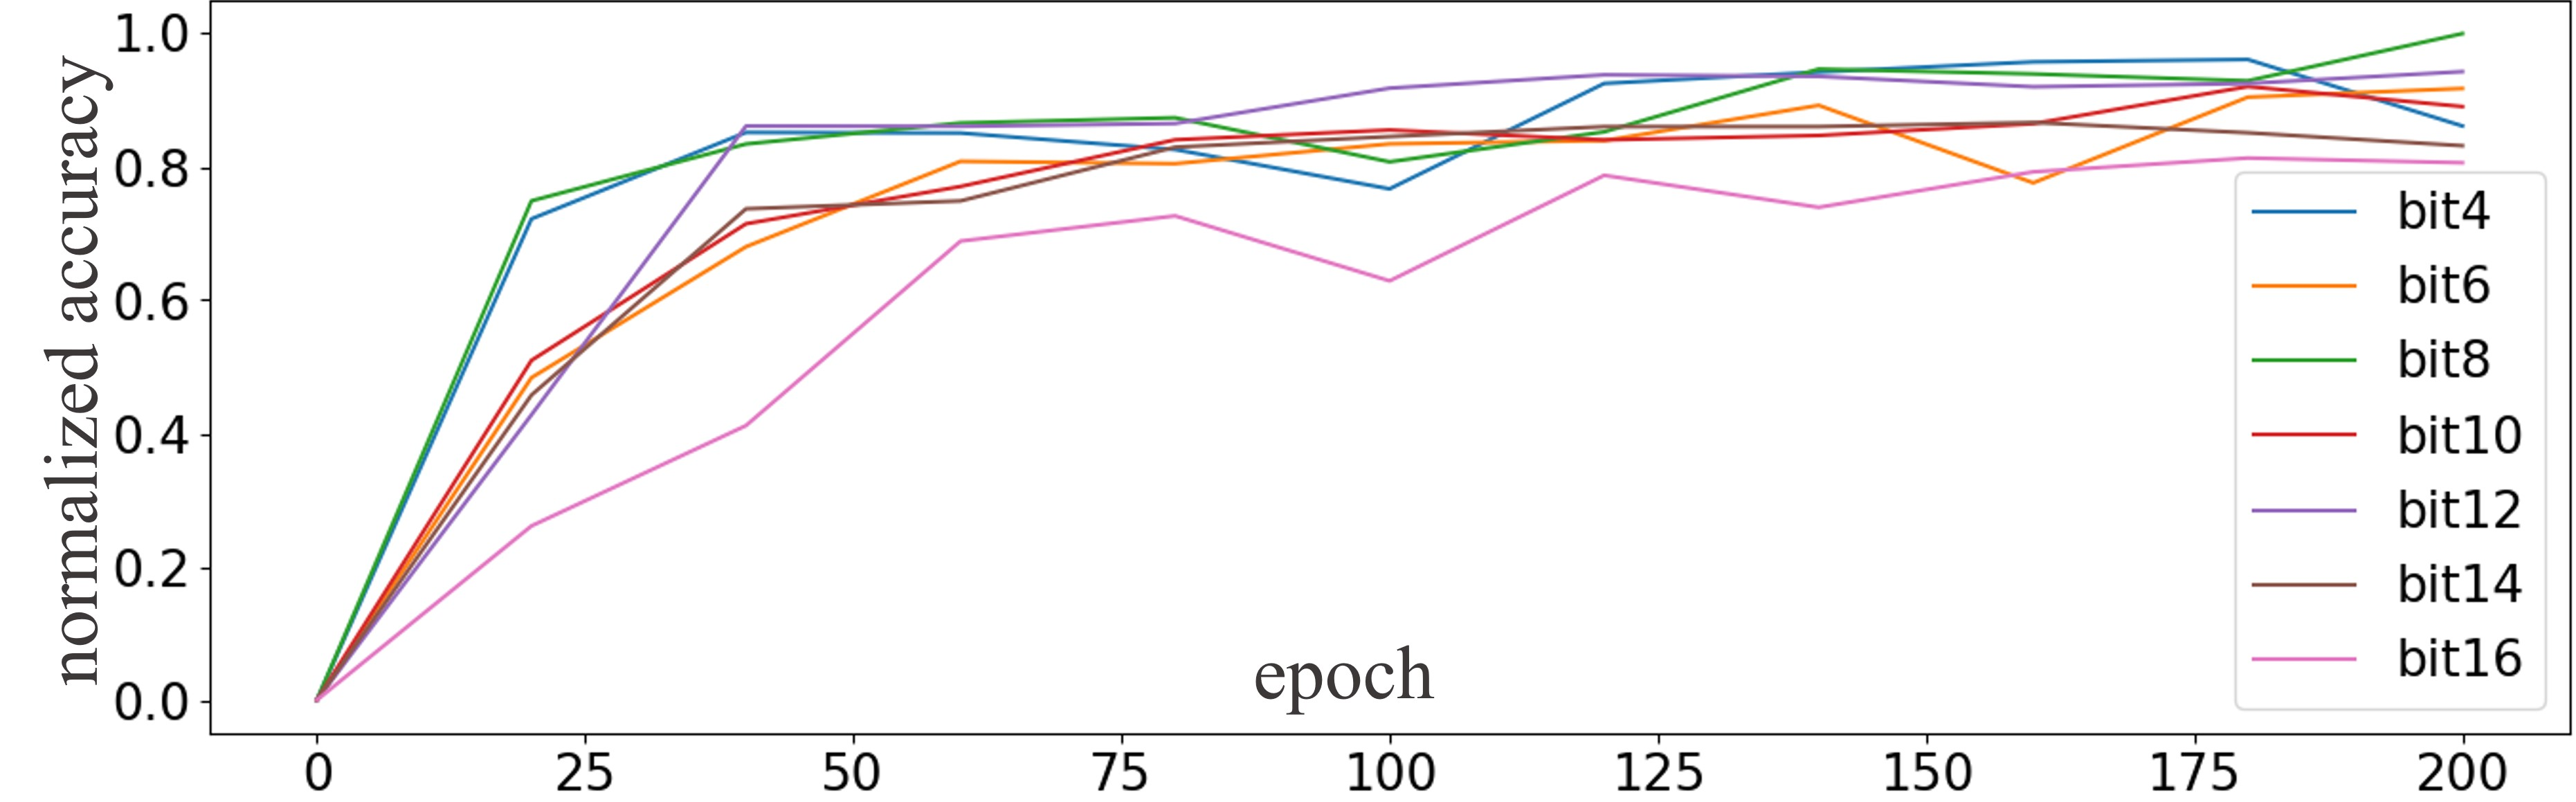
\includegraphics[width=1.0\textwidth]{figure/symnet/ablation_bit.jpg}}
        \caption{T-LESS数据集中obj 27的编码长度$d$对比实验}
        \label{fig:ablation_bit}
\end{figure}

\begin{figure}[ht]
        \centerline{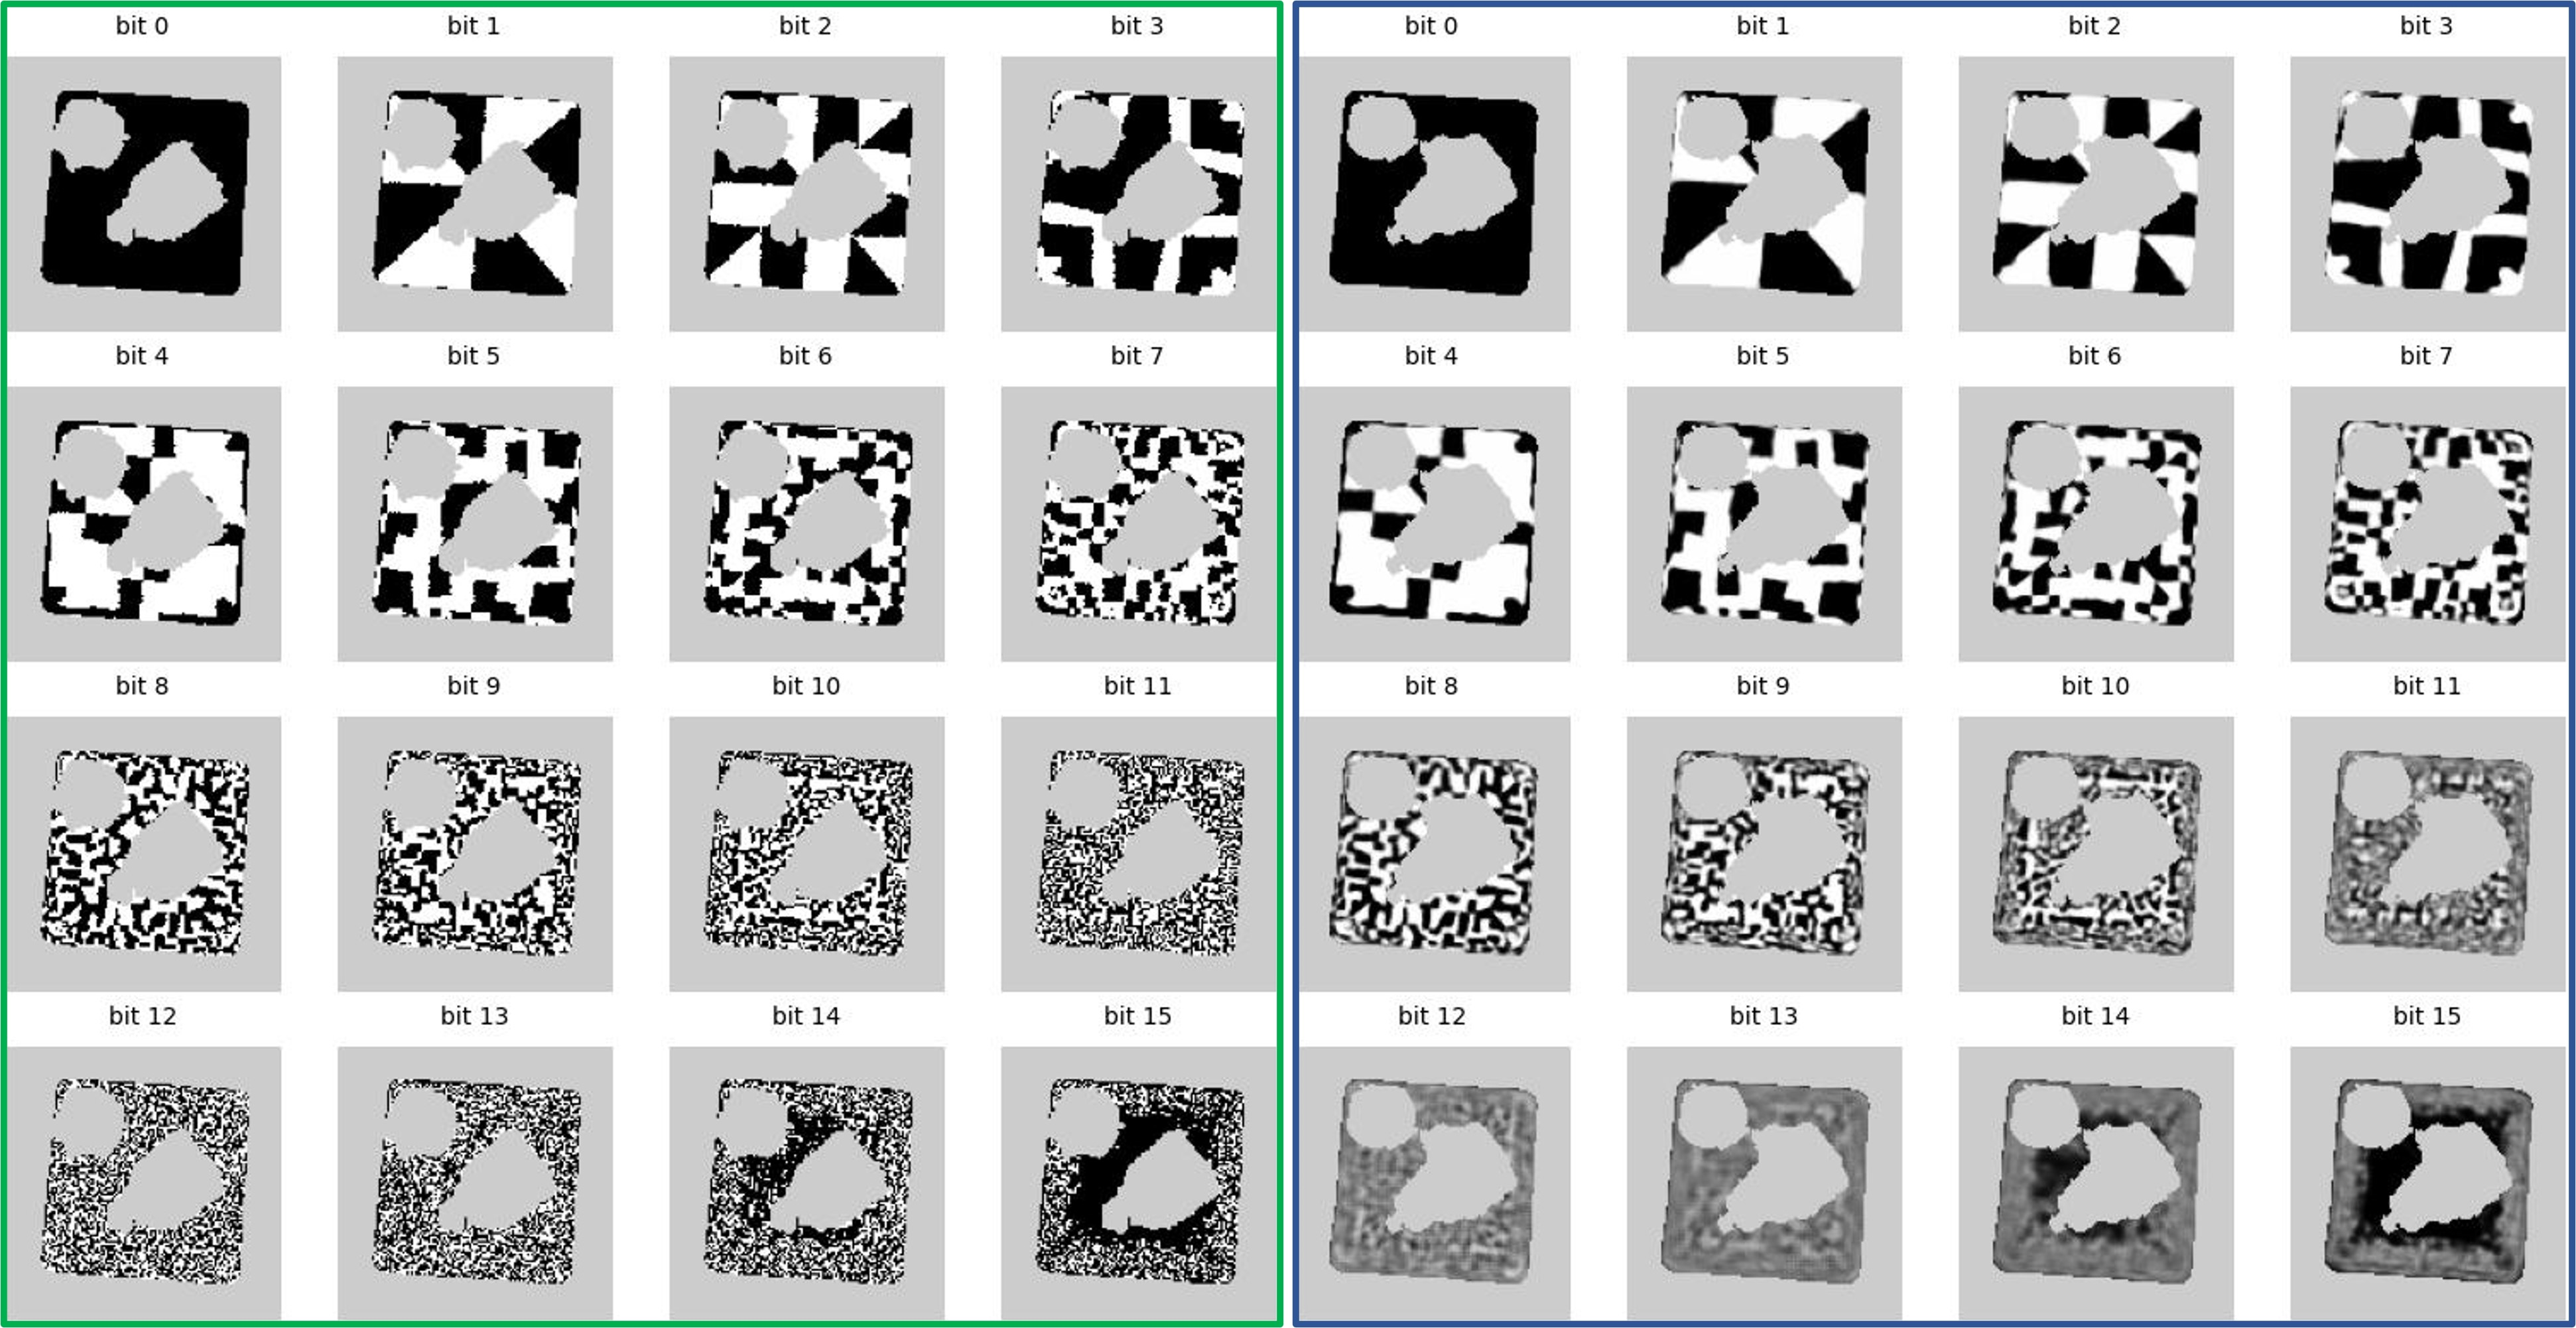
\includegraphics[width=1.0\textwidth]{figure/symnet/compare_gt_est.jpg}}
        \caption{SymCode的真实值和对应学习结果}
        \label{fig:compare_gt_est}
\end{figure}
\textbf{学习一对一对应关系的挑战 } 尝试使用ZebraPose编码训练端到端网络SymNet,这种编码方法旨在有效表示一对一对应关系。
在这种情况下,网络的BOP召回率为0.612,相对于SymNet的0.736表现较弱。当移除所有端到端损失并专注于训练ZebraPose编码时,\autoref{fig:difficult_learn_one_to_one}展示了学习基于一对一对应关系编码的困难。 第一行:具有相似视角的图像。第二行:SymCode的第二位预测结果,对于相似的视角,SymCode的预测结果非常准确。第三行:ZebraPose Code的第二位预测结果,对于相似的视角,ZebraPose Code的预测结果可能出现不一致甚至完全模糊的结果。为实现高精度姿态估计,ZebraPose Code依赖RANSAC-PnP算法过滤不一致的对应关系,但在对称性导致的歧义场景中(如第二列所示)仍存在困难。需要说明的是,该结果使用基于SymNet网络但使用ZebraPose Code进行训练获得。为清晰可视化,采用预测掩码去除背景干扰,并在预测结果中将数值0映射为黑色、1映射为白色,0-1之间的中间值以灰度渐变形式呈现。

\begin{figure}[ht]
    \centerline{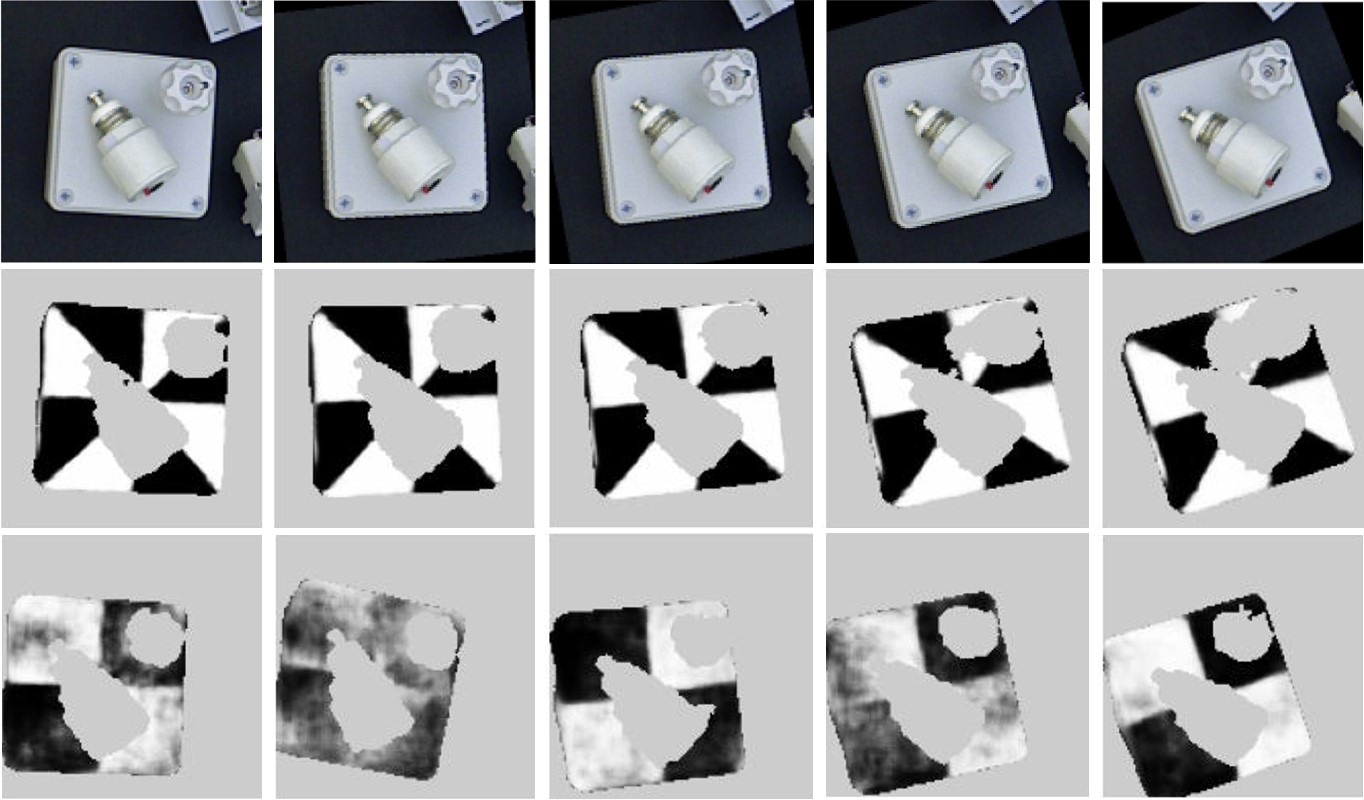
\includegraphics[width=1.0\textwidth]{figure/symnet/difficulty_learn_one_to_one.jpg}}
    \caption{学习一对一对应关系的困难}
    \label{fig:difficult_learn_one_to_one}
\end{figure}

\subsection{可视化} 

\autoref{fig:compare_code_map}通过对比揭示了SymCode与ZebraPose的二进制编码特性差异:首行与第三行呈现ZebraPose编码图,第二行与第四行展示SymCode编码图,末列则为各比特位的聚合可视化结果。该对比清晰揭示了SymCode编码体系对物体对称性信息的有效整合。从\autoref{fig:compare_code_map}观察到ZebraPose编码不具备明显的规律,而SymNet则展现出更优的对称一致性。

\begin{figure}[htbp]
        \centerline{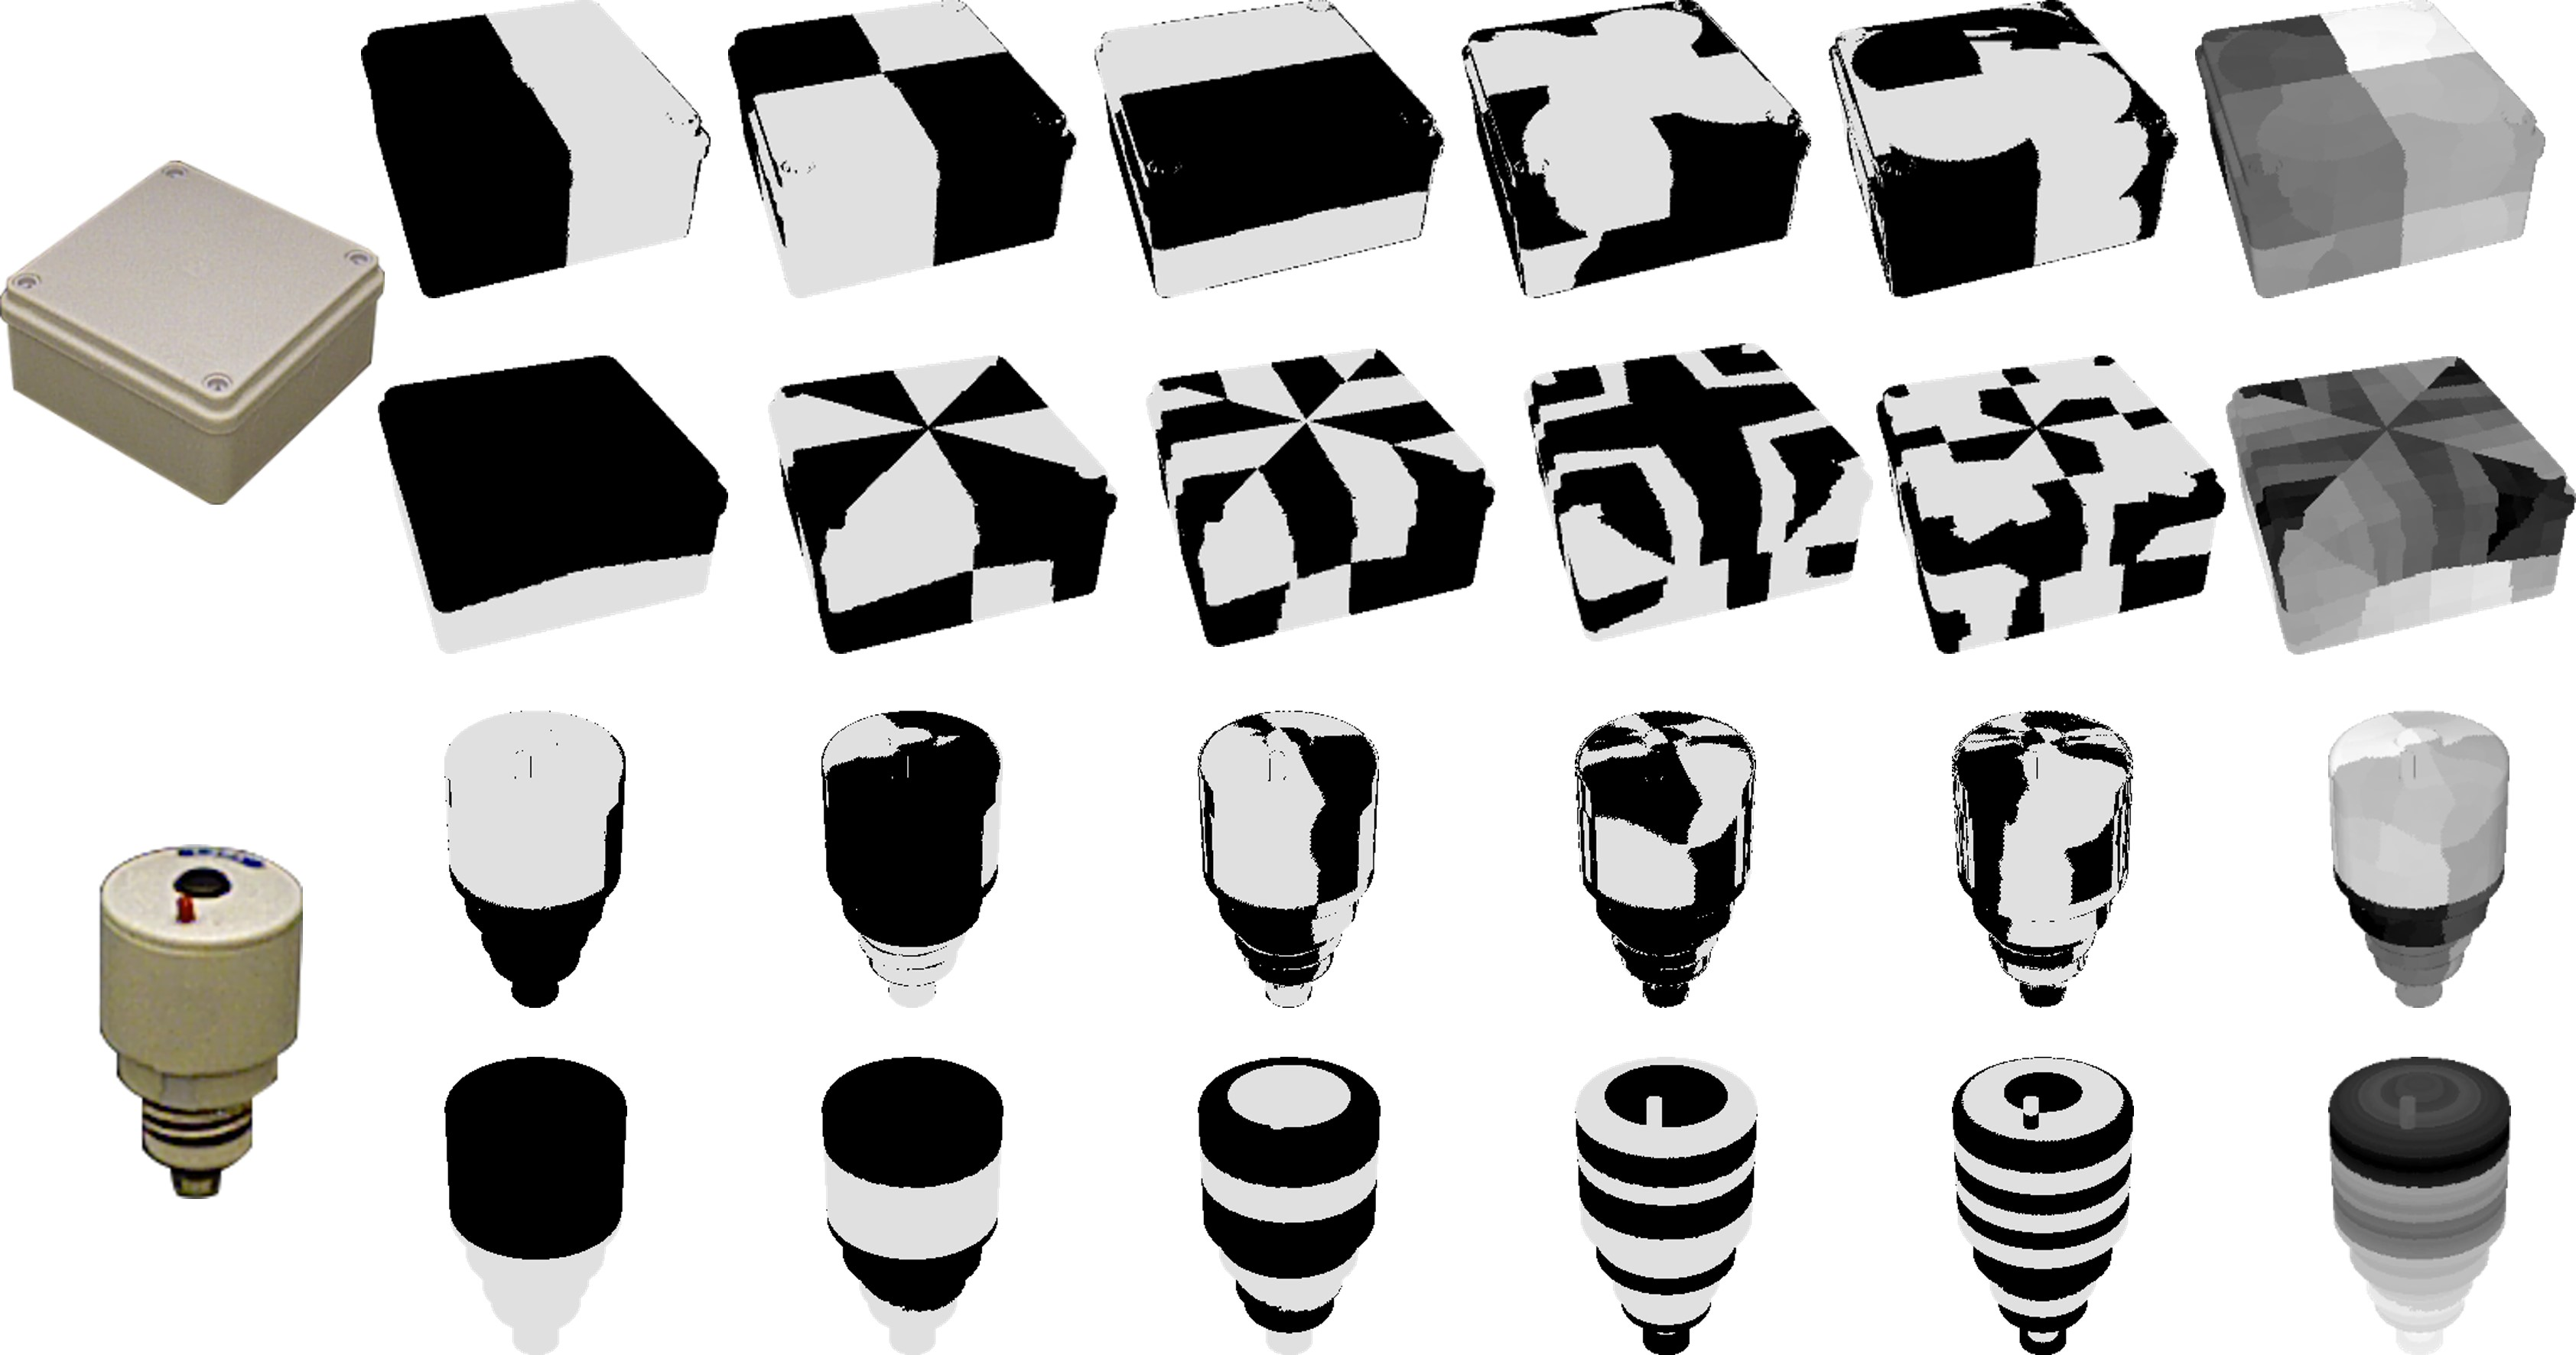
\includegraphics[width=1.0\textwidth]{figure/symnet/compare_code_map.jpg}}
        \caption{ZebraPose Code 和 SymCode 对比}
        \label{fig:compare_code_map}
\end{figure}

\autoref{fig:visualization_tless}展示了在T-LESS数据集上的物体位姿估计结果,两个物体分别为离散对称和连续对称。每列展示不同视角下的场景实例,其中三维物体姿态通过渲染叠加至原始图像。检测置信度分值标注于包围框左上角。可视化结果表明,即使在存在严重遮挡的杂乱场景中,本方法仍能保持鲁棒的姿态估计能力。

\begin{figure}[htbp]
        \centerline{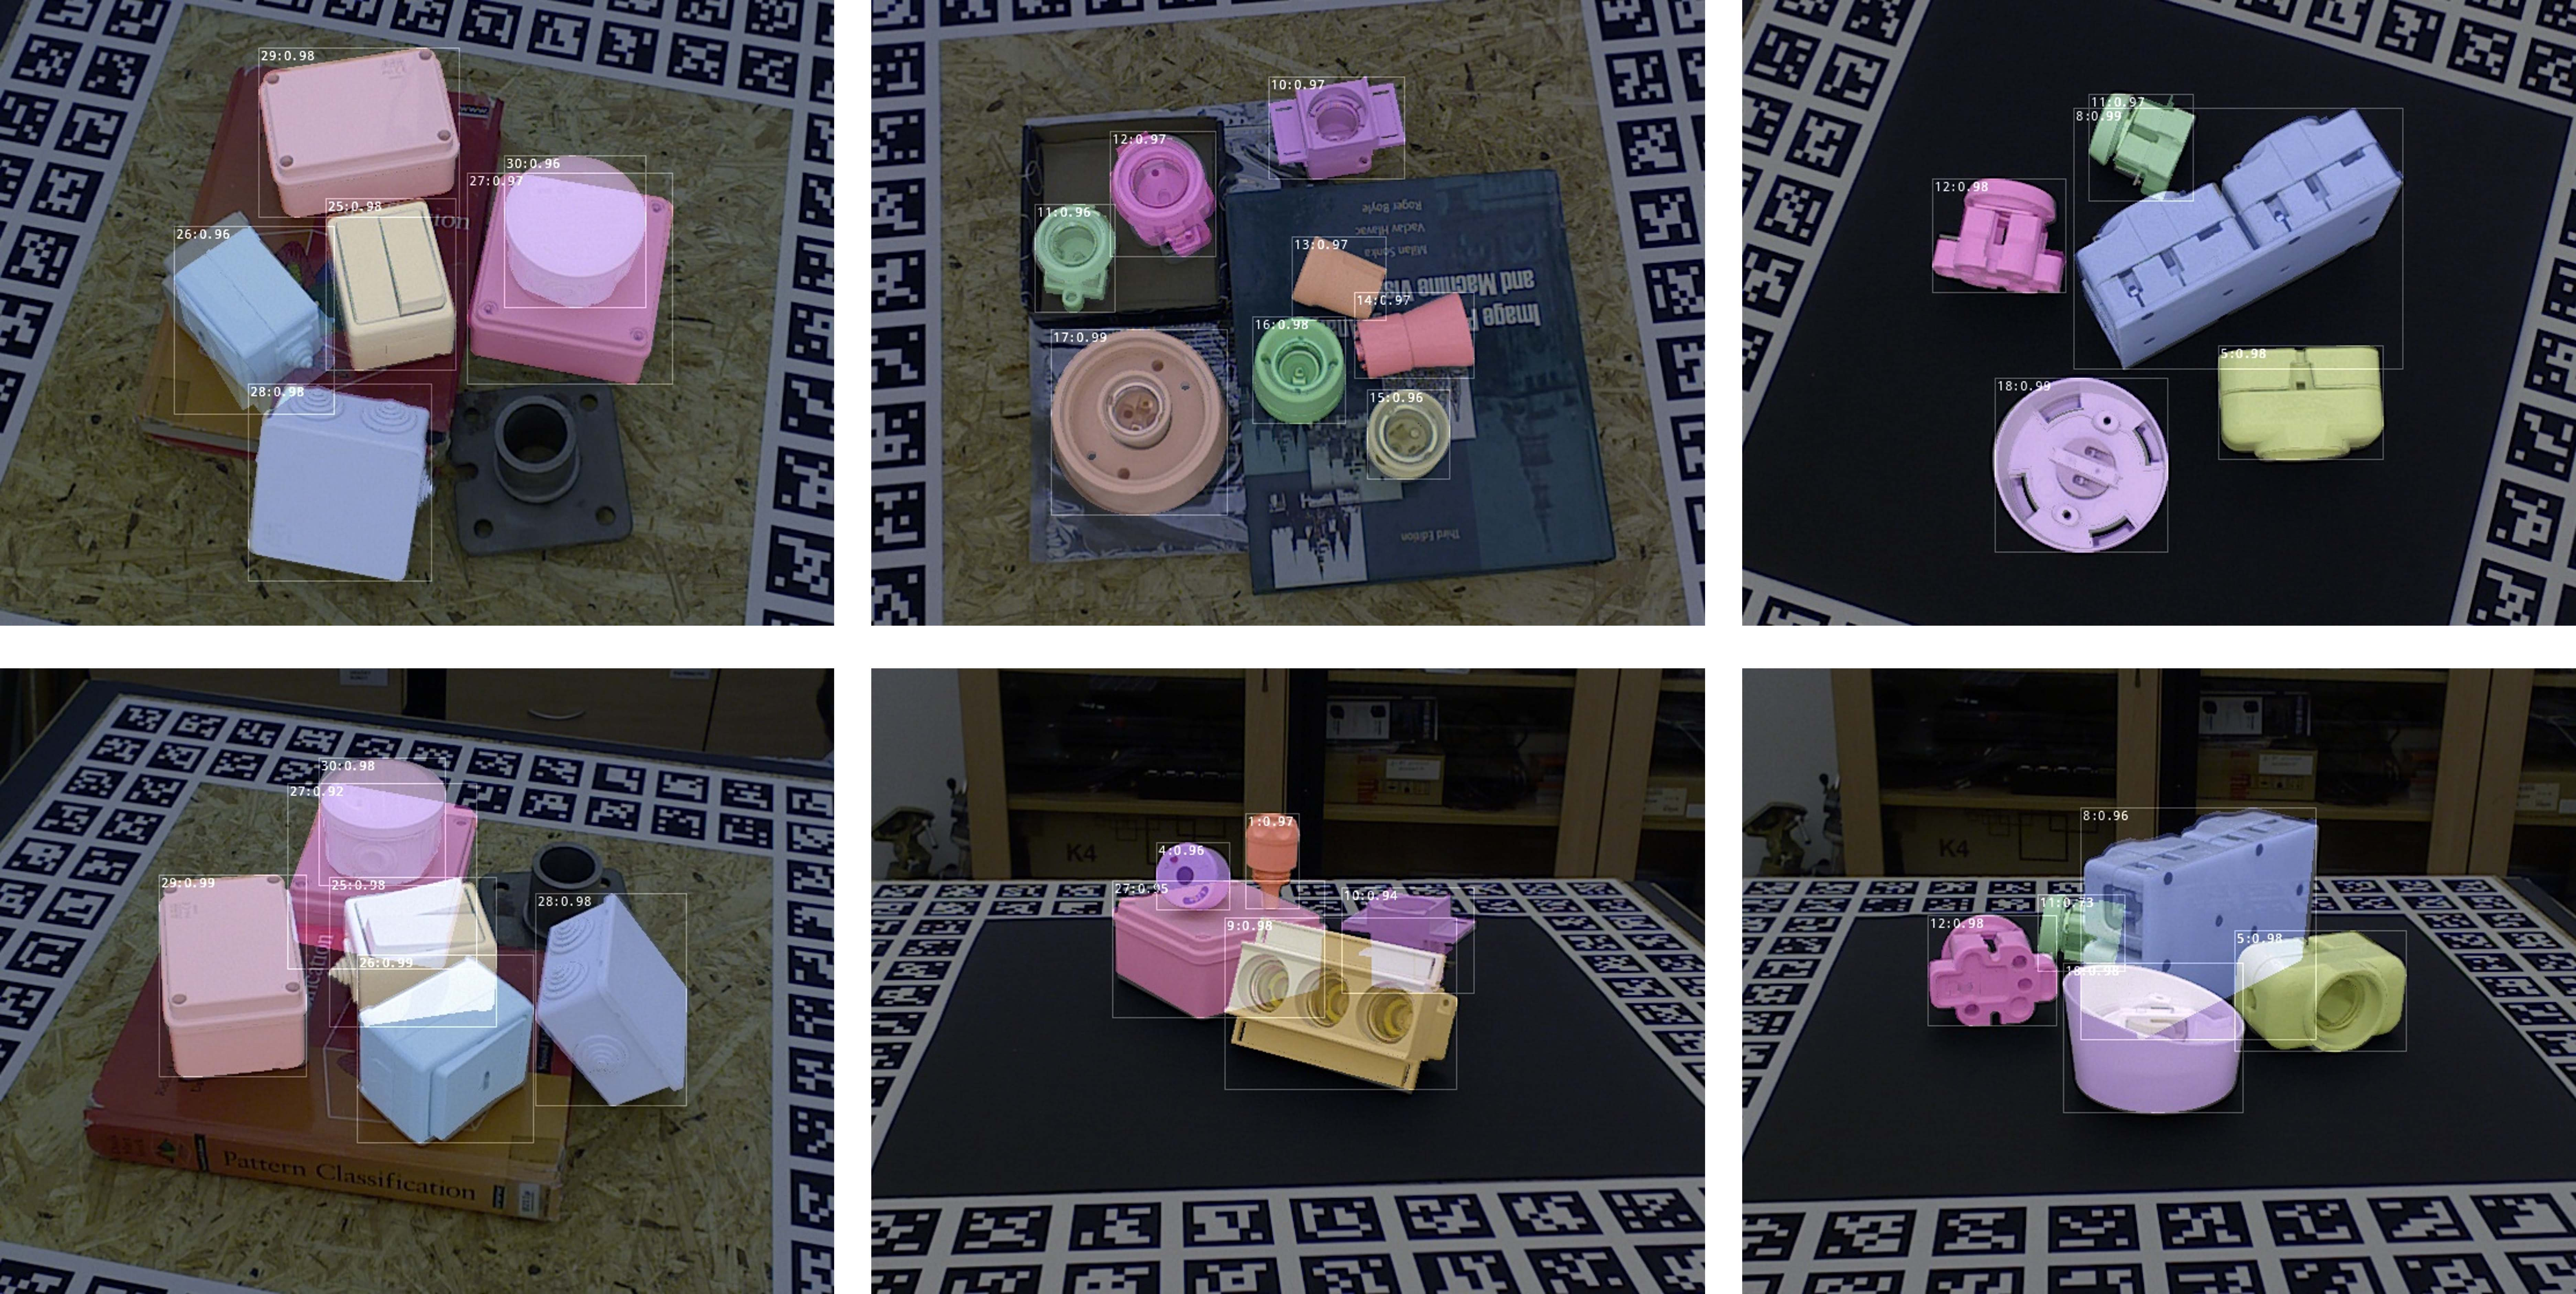
\includegraphics[width=1.0\textwidth]{figure/symnet/visualization_tless.jpg}}
        \caption{在T-LESS数据集上的可视化}
        \label{fig:visualization_tless}
\end{figure}

\autoref{fig:compare_zebrapose}展示了SymCode与ZebraPose Code学习效果对比。左上:ZebraPose的真实值编码;右上:ZebraPose的预测输出;左下:SymCode的真实值编码;右下:SymCode的预测输出(仅显示前8位比特位)。可视化结果表明,SymNet倾向于输出高置信度的预测结果,其预测值常趋近于0或1的极端值域边界。相较而言,ZebraPose的预测值则更多聚集在0.5附近,这种中间态分布揭示了其预测过程存在较高的不确定性,暗示模型对编码空间的表征能力相对不足。

\begin{figure}[htbp]
        \centerline{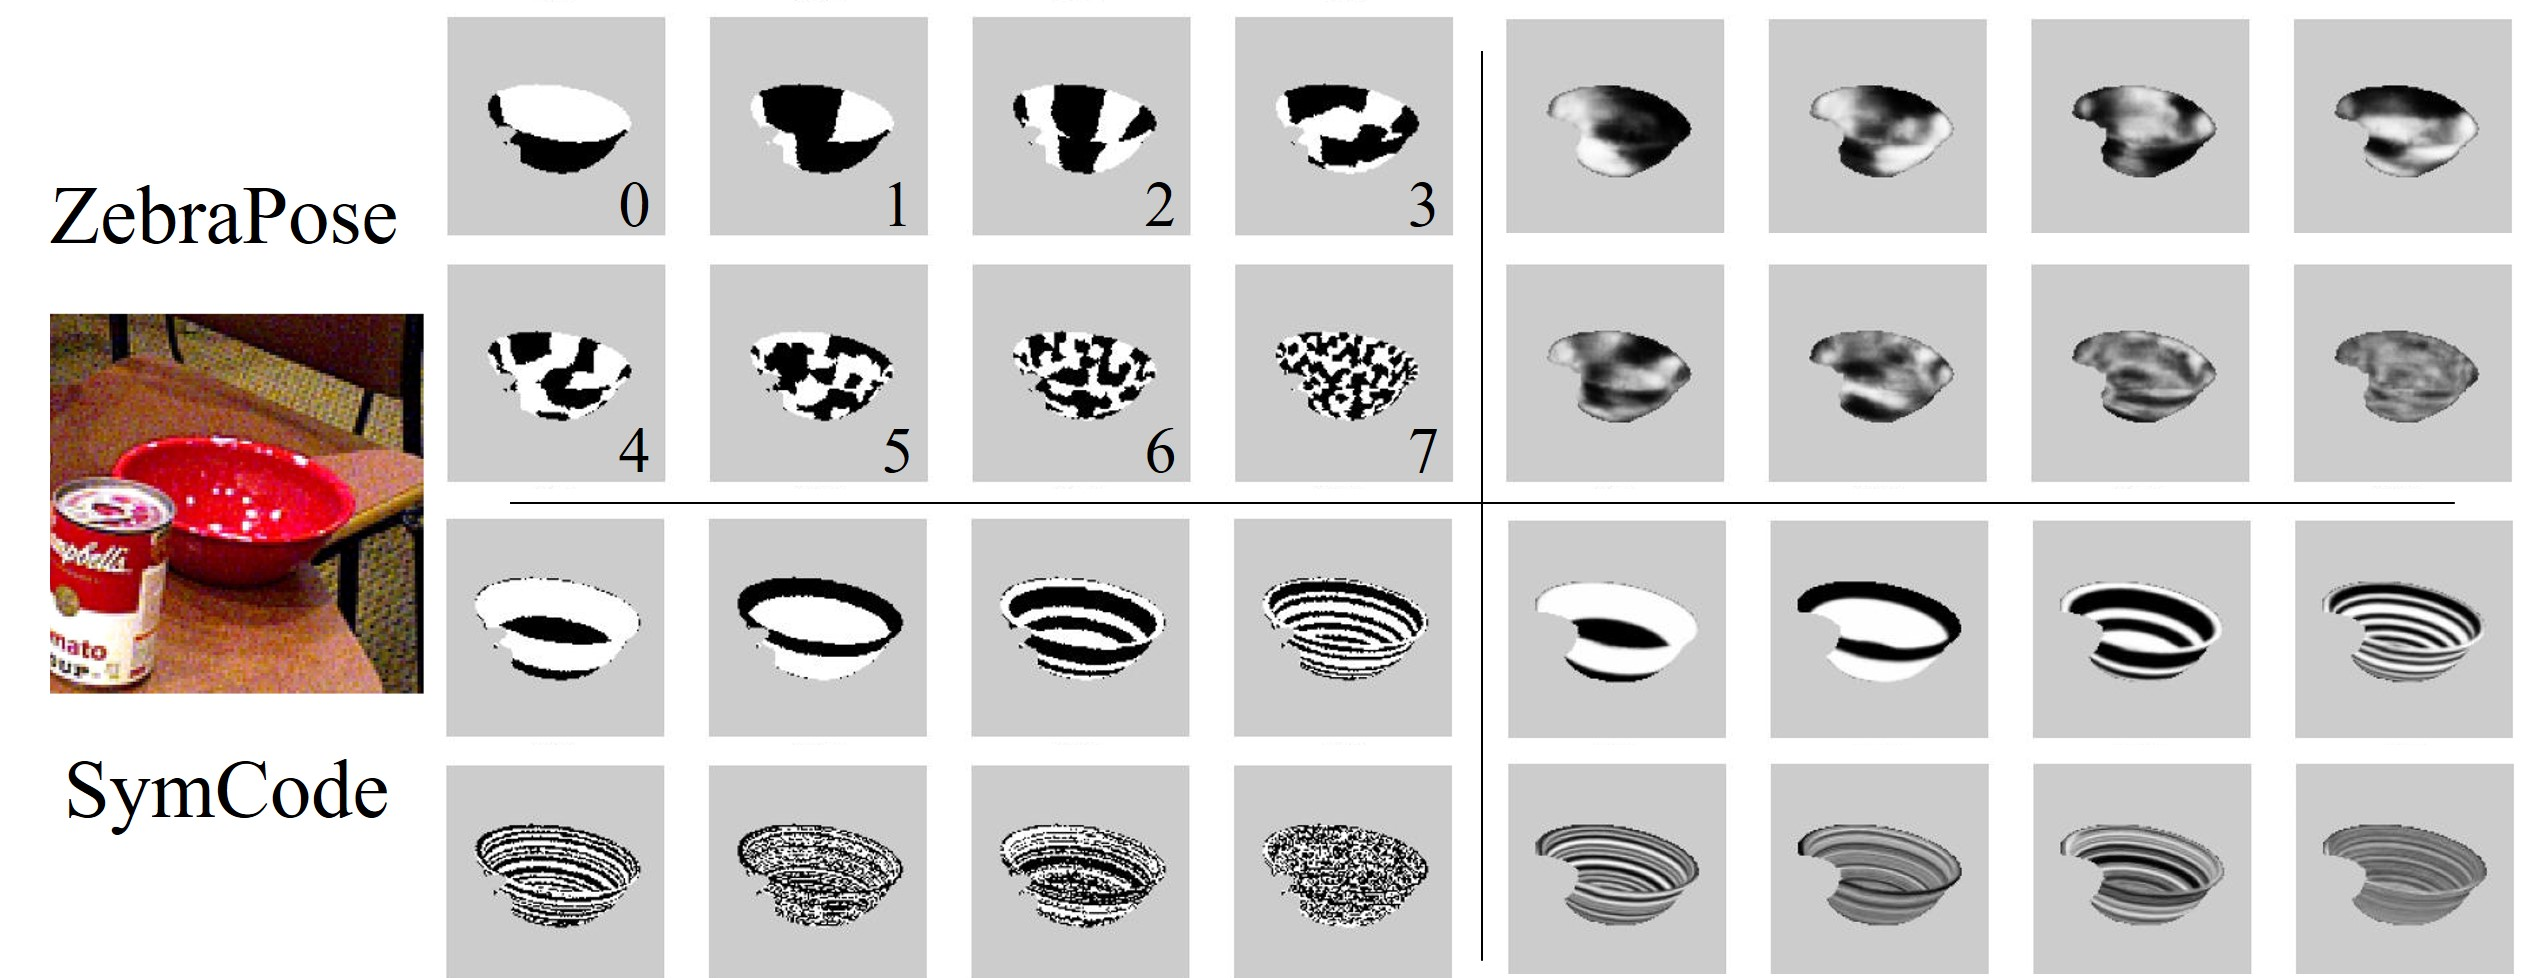
\includegraphics[width=1.0\textwidth]{figure/symnet/compare_with_zebrapose.jpg}}
        \caption{SymCode与ZebraPose Code学习效果对比}
        \label{fig:compare_zebrapose}
\end{figure}

\begin{figure}[ht]
        \centerline{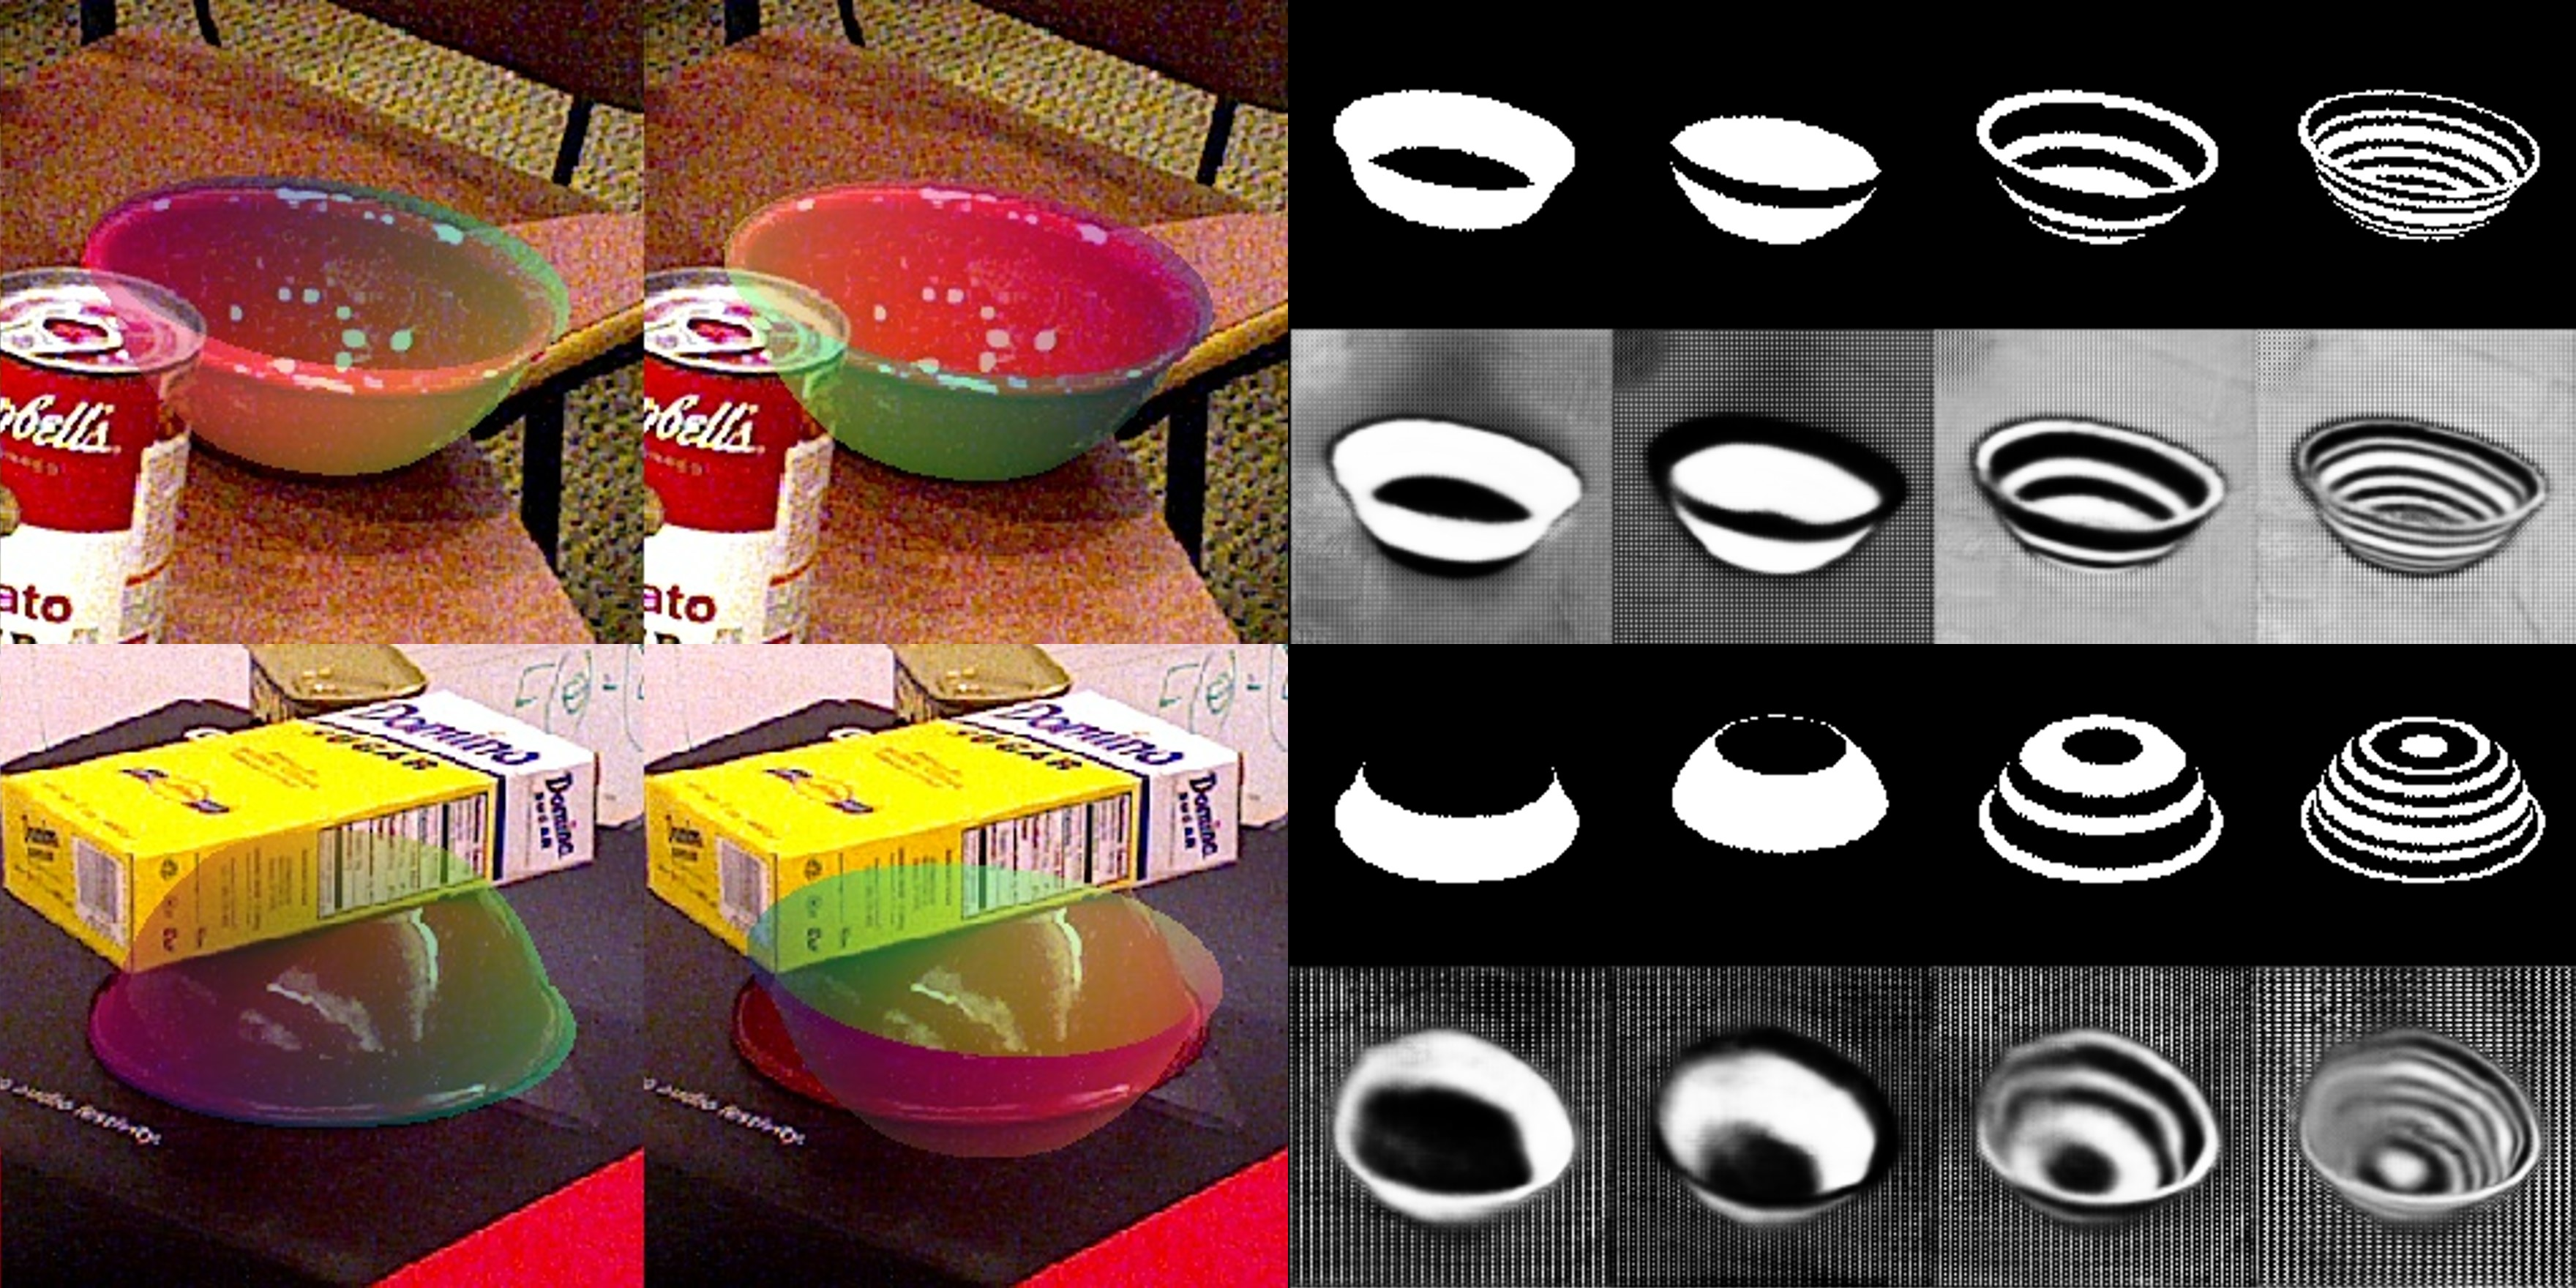
\includegraphics[width=1.0\textwidth]{figure/symnet/ycbv_bowl_vis.jpg}}
        \caption{YCB-V数据集的正确和错误的示例}
        \label{fig:ycbv_bowl_vis}
\end{figure}

进一步可视化了正确和错误的示例,如\autoref{fig:ycbv_bowl_vis}所示。可以发现,在显著遮挡的情况下,输出的二进制编码仍然表现出特定姿态的特征,尽管该姿态是错误的。第一列为真实值,第二列为估计的姿态。第一个示例是正确估计的情况,而第二个示例是错误估计的情况。右侧的第一行和第三行为SymCode的真实值,第二行和第四行为估计值。

